\documentclass{article}
\usepackage{amsmath}
\usepackage{enumerate}
\usepackage{listings}
\usepackage{moreverb}
\usepackage[margin=1in]{geometry}
\usepackage{graphicx}
\usepackage{dsfont}
\title{STA 360: Assignment 7}
\author{Michael Lin}

\begin{document}
\maketitle


\begin{enumerate}[7.1]
	\setcounter{enumi}{2}
	\item
	\begin{enumerate}[(a)]
		\item The posterior samples of $\mathbf{\theta}$ and $\Sigma$ are obtained using a Gibbs sampler based on the full conditionals derived in Hoff. Here are the full conditional for $\theta$:
		$$\mathbf{\theta}|y_1, y_2, \Sigma \sim \text{MVN}(\mu_n, \Lambda_n)$$
		where
		$$\mu_n = (\Lambda_0^{-1}+n\Sigma^{-1})^{-1}(\Lambda_0^{-1}\mu_0+n\Sigma^{-1}\bar{y}) $$
		$$\Lambda_n = (\Lambda_0^{-1}+n\Sigma^{-1})^{-1} $$
		and the full conditional for $\Sigma$:
		$$\Sigma|y_1, y_2, \theta \sim \text{IWish}(\nu_n, S_n^{-1})$$
		where
		$$\nu_n = \nu_0 + n$$
		$$ S_n = S_0 + \sum\nolimits_{i} (y_i-\theta)(y_i-\theta)^T$$
		For the Gibbs sampler, we set:
		$$ \mu_0 = \bar{y}$$
		$$\Lambda_0 = S_0 = \Sigma_{y_1, y_2}$$
		and we set the starting point:
		$$\Sigma^{(0)}=S_0 $$
		
		\item Bivariate distribution plot of $\theta$'s for blue and orange crabs:
		
		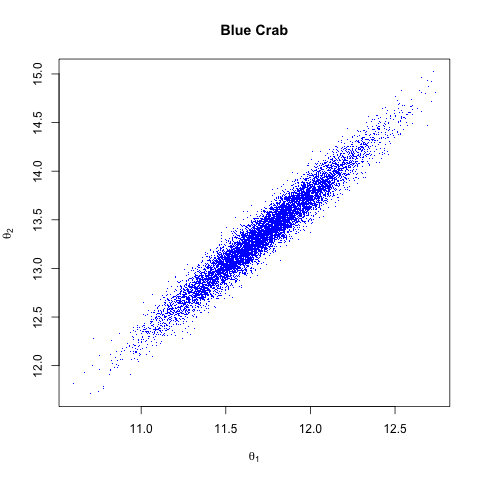
\includegraphics[scale=0.4]{bluetheta.png}
		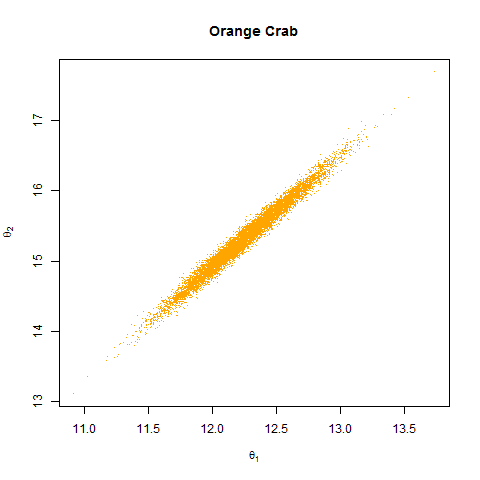
\includegraphics[scale=0.4]{ortheta.png}
		
		The plots suggest that while orange crabs on average have slightly larger body depth than blue crabs, orange crabs have significantly larger rear width than blue crabs.
		
		\item Posterior density plots of the correlations $\rho_{\text{blue}}$ and $\rho_{\text{orange}}$:
		
		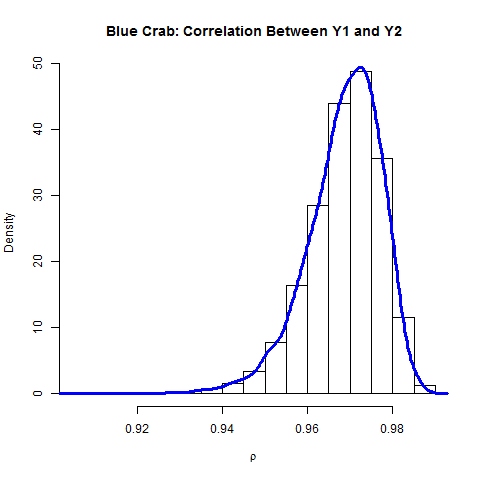
\includegraphics[scale=0.4]{bluedist.png}
		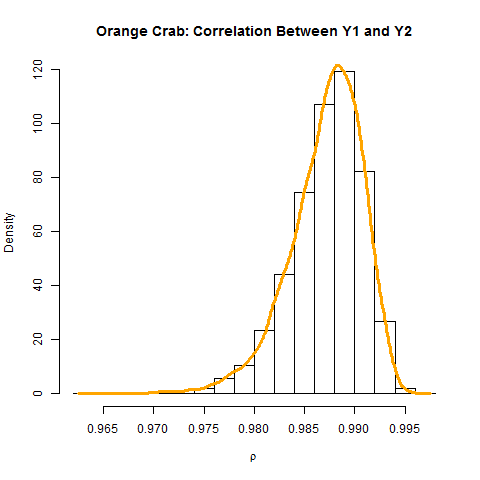
\includegraphics[scale=0.4]{ordist.png}
		
		A comparison of correlation coefficients from each update of the Gibbs sampler yielded approximately that:
		 $$\text{Pr}(\rho_{\text{blue}}<\rho_{\text{orange}}|y_{\text{blue}}, y_{\text{orange}}) \approx 0.9908$$
		 The plots show that the distribution of correlations between body depth and rear width for orange crabs has a smaller range and higher mean. These results suggest that body depth and rear width are more correlated for orange crabs, and that orange crabs are more similar to one another than blue crabs.
		
	\end{enumerate}
	
	\setcounter{enumi}{4}
	\item
	\begin{enumerate}
		\item Below are empirical estimates based on the data:
		\begin{align*}
			\hat{\theta}_A = 24.200 \\
			\hat{\theta}_B = 24.805 \\
			\hat{\rho} = 0.616 \\
			\hat{\sigma}_A^2 = 4.093 \\
			\hat{\sigma}_B^2 = 4.692
		\end{align*}
		
		\item Using paired t-test on $A$ and $B$ responses, a $t$-value of -3.2807 was obtained with a $p$-value of 0.00177. As a result, we reject the null hypothesis and conclude that $\theta_A<\theta_B$. A 95\% confidence interval for $\theta_A-\theta_B$ is [-0.9851, -0.2383].
		
		\item After implementing a Gibbs sampler with a unit information prior, a posterior mean for $\theta_A-\theta_B$ is -0.6730. A 95\% confidence interval for $\theta_A-\theta_B$ is [-1.1210, -0.2250].
	\end{enumerate}
\end{enumerate}

\pagebreak
R code for 7.3:
\listinginput[1]{1}{crab.r}

\pagebreak
R code for 7.5:
\listinginput[1]{1}{imputation.r}
\end{document}